%!TEX root = main.tex

\section{Analysis of Web Search}
\label{sec:web_search}

\begin{figure}[th]
\centering
	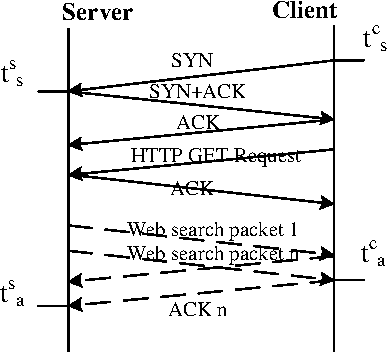
\includegraphics[width=0.5\linewidth]{web_finish_time_example}
\caption{Time-line in web search flow.}
\label{fig:web_finish_time_example}
\end{figure}

Web search starts when mobile terminal initiates connection to transmit query text, and ends when server receives ACKs for all returned search results. Figure~\ref{fig:web_finish_time_example} shows the typical time-line in web search flows. The finish time at client side is the duration from transmitting SYN packet $t^c_s$ to receiving all web search data $t^c_a$. We use the duration $T_s=t^s_a - t^s_s$ measured at server side to approximate the latency that user perceives. Again, we excluded the time consumed by servers processing the query $T_r=t^s_r - t^s_q$ and obtained the finish time as $T_s-T_r$.

\begin{figure}[th]
\centering
	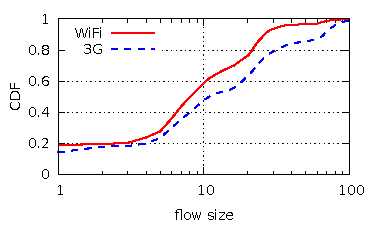
\includegraphics[width=0.8\linewidth]{web_flow_size}
\caption{The distribution of flow sizes in web search.}
\label{fig:web_flow_size}
\end{figure}

Figure~\ref{fig:web_flow_size} plots the distribution of flow size (measured by the number of web search result packets) in web search. The flow size varies from 1 packet to 100 packets with a median around 10 packets. Such a small flow size implies that any TCP performance degradation (like a high packet loss) could exert a large impact on the user perceived latency (i.e. finish time) \cite{flach2013reducing}. We also observe a smaller flow size of WiFi search than that of 3G search, which might be due to the difference in search behavior \cite{Song:2013:EEU:2488388.2488493}. We use Kendall correlation to determine whether flow size is relevant to finish time. The coefficient is 0.018, which demonstrates their irrelevance. Here we also investigate the relationship between finish time and RTT. The distribution of RTT in web search is similar to that in voice recognition, which is not shown due to space limit. The coefficient between RTT and finish time is 0.15, showing weak relationship between them. The reason is as follows. Web search result should be transmitted in several RTT's. The congestion window, which determines how many packets are transmitted in one RTT, could be reduced by half due to packet loss, and increased twice if no packet loss in the RTT. Thus RTT has limited impact on finish time in web search. 

As a TCP sender in web search, the server can measure abundant TCP performance factors and behavior, enabling us to perform a detailed analysis of the TCP performance and its impact on the finish time. In what follows, we first characterize the finish time distribution in 3 TCP stages and then examine the impact of TCP performance factors.


%The flow size in web search ranges from 1 to 100 packets. This means that the data could be transmitted in 1 RTT at least, and more than 4 RTT at most. Considering the various flow sizes, the metric $finish\_time$ could not portray the efficiency that the data is delivered. To eliminate the affect of flow size, we introduce one more performance metric transmission time per packet ($tpp$), defined as the average time to transmit a data packet. The metric $tpp$ could be represented as $\frac{finish\_time}{\#(pkts)}$. In the following, we mainly use transmission time per packet ($tpp$) to depict the performance of web search.

\subsection{TCP Stage Anaysis}

\begin{figure}[th]
\centering
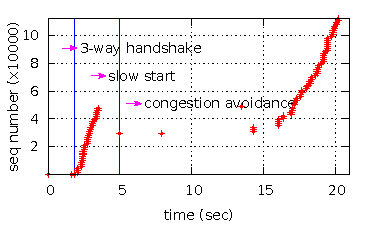
\includegraphics[width=0.8\linewidth]{web_three_stages}
\caption{The three stages in web search flows.}
\label{fig:web_three_stages}
\end{figure}

A TCP comprises 3 stages: \emph{3-way handshake}, \emph{slow start}, \emph{congestion avoidance}, which is exemplified in Figure~\ref{fig:web_three_stages} using a web search flow from our dataset, where $y$-axis shows the TCP sequence number. The TCP 3-way handshake (3WHS) stage ideally (i.e. without packet loss, delay and reordering) completes within 1 RTT. The server then enters the slow start stage, during which server does not encounter any packet loss or reordering event, and thus enlarges the congestion window by 1 segment size for each received ACK. The server enters congestion avoidance stage once it estimates a packet loss\footnote{The packet can actually be delayed or lost.}. In this stage, the server reduces the congestion window when detecting packet loss through fast retransmit\cite{jacobson1988congestion} and compels the congestion window to grow from 1 segment size when detecting packet loss through RTO. Note that the congestion avoidance stage here starts when server detects congestion event and ends till the flow finishes, which is different the TCP congestion avoidance state in TCP/IP stack. 



%Figure~\ref{fig:web_three_stages} gives an exemplified flow with 3 TCP stages that we define. The $y$-axis shows the TCP sequence number. In the figure, server takes 1.8s to establish connection, 3.1s to transmit 35 data packets in slow start stage, and 15.3s to transmit the left 48 data packets in congestion avoidance stage. In the following, we use the criteria of partitioning to break the analysis down into the three stages that flows experience.

\subsubsection{3-way Handshake}

\begin{figure}[th]
\centering
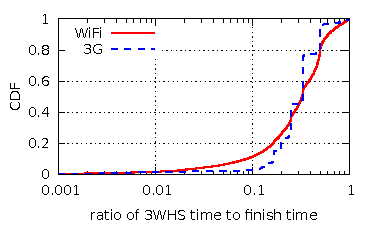
\includegraphics[width=0.8\linewidth]{web_handshake_time_ratio}
\caption{The ratio of time in 3-way handshake to finish time in each flow.}
\label{fig:web_handshake_ratio}
\end{figure}

We first examine how much of the time spent in the 3WSH stage in Figure~\ref{fig:web_handshake_ratio}, where we plot the ratio of the time in 3WSH to the finish time. 3G and WiFi show similar ratio of time spent in this stage. We observe that the time for connection establishment can take up to half of the finish time for 30\% flows. More surprisingly, about 8\% of the WiFi flows and 3\% of 3G flows spend 70\% of their time during this stage. The small flow size is one of the reason for this observation. The maximum flow size is around 100 packets as shown in Figure \ref{fig:web_flow_size}, implying the data can be transmitted within only a few RTTs if no congestion event happens. such a short period of transmission time leads to a relatively large portion of time for connection establishment.


%From the figure, flows in cellular network have similar ratio of time in 3-way handshake to that in WiFi network (with median value 0.3). If the 3WSH could be removed from finish time, the user-perceived web search latency would be reduced by 30\% in more than half of the flows. Moreover, there are 8\% of flows in WiFi network consuming 70\% of their time in 3WSH.

%The unexpectedly high ratio of 3WSH could be introduced by two reasons. First, most of web search flows contains packets ranging from 1 to 100, these data could transmitted in 1 to 4 RTT's if there is no congestion event. Thus 3WHS, without transmitting any data, occupies a large fraction of time in short flows. Second, there are a non-negligible fraction of flows experiencing SYN retransmission during 3WHS stage. 

Another important reason that explains the unexpectedly the long time in 3WSH stage (i.e. $>70\%$ of finish time) is the timeout retransmissions in this stage. As the data cannot be transmitted before a TCP connection is established, a loss of SYN will lead to a timeout retransmission, which takes 1 second (\ie the initial RTO) to retransmit the SYN.  We find that 4.4\% of WiFi search flows and 0.5\% of 3G flows experience at least one SYN timeout retransmission. We envision a possible way to mitigate the costly 3WSH in such short flows where clients maintain long-term TCP connections to the web search servers.

%\begin{table}[th]
%\centering
%\renewcommand{\arraystretch}{1.1}
%\caption{Percentage of flows that experience SYN retransmission in web search.}
%\label{tab:web_syn_retrans}
%\begin{tabular}{l|c|c|c}
%\toprule
%& WiFi & 2G & 3G \\
%\midrule
%SYN retransmission & 4.4\% & 2\% & 0.5\% \\
%\bottomrule
%\end{tabular}
%\end{table}

\subsubsection{Slow Start Stage}

\begin{figure}[th]
\centering
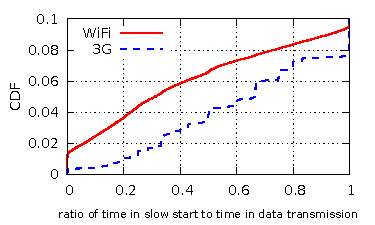
\includegraphics[width=0.8\linewidth]{web_slowstart_time_ratio}
\caption{The ratio of time in slow start to the time in data transmission.}
\label{fig:web_ss_time_ratio}
\end{figure}

The slow start stage and the congestion avoidance stage constitute the data transmission period. During the slow start stage, the data transmission throughput monotonically increases as the congestion window is doubled after each RTT. Intuitively, a longer time in slow start stage, the shorter time to complete the data transmission. Figure~\ref{fig:web_ss_time_ratio} shows the ratio of time in slow start stage to the time spent in data transmission (\ie the sum of time in slow start and congestion avoidance stages). Note that the $y$-axis is capped at 0.1. Regardless of the access type, more than 90\% of the flows can be finished in the slow start stage. In other words, about 10\% of the flows have to experience the congestion avoidance stage, which could lead to an increased finish time as we will see in the following analysis.

Another interesting observation is that 1.5\% of the WiFi flows is unable to transmit any data in the slow start stage as the first packet is dropped. We indeed find of the flows that experience the congestion avoidance stage, the packet loss happens within the first congestion window (i.e. within the first 10 packets) for 80\% of WiFi flows, while this percentage is only 20\% for 3G flows, implying a reconsideration of the initial congestion window configuration.

%This is an evidence that increasing initial congestion window to 10 segment size is not always helpful to all flows.

%In the figure, 8\% - 10\% of flows could not transmit all the web search data in slow start stage, which is also the percentage of flows experiencing packet loss. Moreover, 6.5\% of flows in WiFi network and 4\% of flows in cellular network could only spend half of their transmission time in slow start stage. Particularly, 4\% of flows in WiFi network could not transmit any data in slow start stage, in which the first packet is dropped.
%
%\begin{figure}[th]
%\centering
%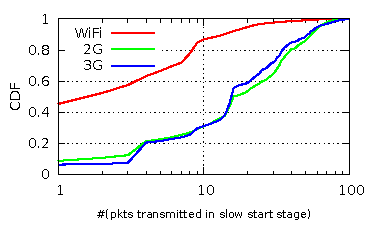
\includegraphics[width=0.8\linewidth]{web_slowstart_pkts}
%\caption{Number of packets transmitted in slow start stage.}
%\label{fig:web_ss_pkts}
%\end{figure}
%
%Figure~\ref{fig:web_ss_pkts} shows the distribution of packets which could be transmitted in slow start stage. In the figure, only these flows experiencing packet loss are considered. In the considered flows, flows in WiFi network could transmit less data packets in slow start stage than those in cellular network. This could be induced by higher packet loss rate in WiFi network, which we will investigate in Section~\ref{sec:web_pkt_loss}. In particular, 85\% of the considered flows (\ie 8.1\% of all flows) in WiFi network experience packet loss in the initial congestion window. This is an evidence that increasing initial congestion window to 10 segment size is not always helpful to all flows.

\subsubsection{Congestion Avoidance Stage}

%\begin{figure}[th]
%\centering
%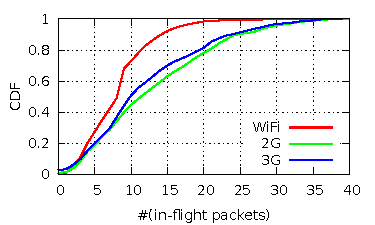
\includegraphics[width=0.8\linewidth]{web_ca_inflight}
%\caption{Number of in flight packets when flows entering congestion avoidance stage.}
%\label{fig:web_ca_inflight}
%\end{figure}
%
%Figure~\ref{fig:web_ca_inflight} shows the distribution of in flight packets when flows enter congestion avoidance stage. In the figure, only these flows experiencing packet loss are considered. In flight packets are those estimated in the network (\ie not dropped) yet not acknowledged by the receiver. When encountering packet loss, the number of in flight packets could be regarded as the number of packets allowed by network that could be transmitted in one RTT. In the figure, 80\% of flows in WiFi network have no more than 12 in flight packets. In contrast, 80\% of flows in cellular network have no more than 20 in flight packets. Flows in WiFi network have smaller in flight size than those in cellular network. This means that WiFi network allocates lower bandwidth for flows than cellular network.

\begin{figure}[th]
\centering
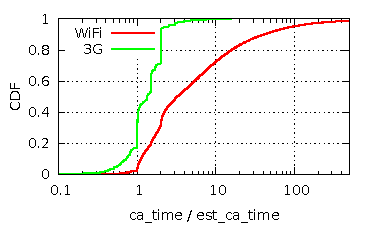
\includegraphics[width=0.8\linewidth]{web_ca_prac_over_est}
\caption{CDF of the extra time introduced by the congestion avoidance stage.}
\label{fig:web_ca_round}
\end{figure}

We then examine how much extra time the congestion avoidance stage introduces for individual flows. To this end, we first compute an estimated ideal transmission time ($T_e$) without this stage for each flow. The estimated ideal time is $T_e = \frac{\#(ca\_pkts)}{cwnd} \times RTT$, where $\#(ca\_pkts)$ is the number of packets transmitted in this stage, $cwnd$ is the congestion window size at the server at the time when entering this stage. However, we cannot obtain $cwnd_e$ from the traces and thus alternatively use the number of in-flight packets at the time when entering the stage to approximate $cwnd_e$ \cite{rfc56812009tcp}. Then we compute the ratio of the time spent in this stage obtained from the trace (denoted as $T_r$) to the estimated idea transmission time. We use this ratio to measure the extra time introduced by the congestion avoidance stage and show the results in Figure \ref{fig:web_ca_round} for those flows experiencing this stage.

We observe a surprisingly high ratio for WiFi flows. The median ratio is as high as 3.2 and 20\% of the WiFi flows has a ratio more than 11, meaning a 10 times extra time is introduced by this stage. The high ratio can be attributed to two factors. First, the real congestion window of these flows is much smaller than $cwnd_e$ due to packet losses. Second, some lost packets require the timeout retransmission to recover, in which cases server must wait for a RTO without data transmission. It is interesting to see that 3G flows have a ratio no more than 2 for 95\% of the flows, meaning that 3G flows have a low packet loss rate and experience fewer timeout retransmissions. In what follows, we will examine in detail the impact of packet loss and timeout retransmission on finish time. 

\subsection{Impact of packet loss}
\label{sec:web_pkt_loss}

\begin{figure}[th]
\centering
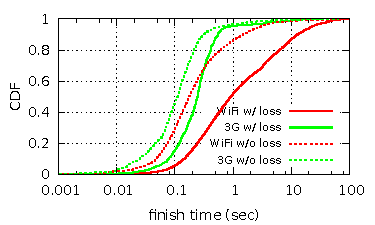
\includegraphics[width=0.8\linewidth]{web_loss_fintime_cdf}
\caption{The distribution of finish time with and without packet loss in web search.}
\label{fig:web_loss_fintime_cdf}
\end{figure}

As we have analyzed above, packet loss would degrade TCP performance by both reducing congestion window and possibly triggering timeout retransmission. The the web search dataset, about 9\% of flows in both WiFi and cellular network experience packet loss. However, the packet loss rates in WiFi and cellular network are 3\% and 0.9\% respectively. Figure~\ref{fig:web_loss_fintime_cdf} shows the distribution of finish time with and without packet loss in web search. In the figure, there are distinct performance gap between flows with and without packet loss. The mean finish time in flows without packet loss is about 2.5 - 5 times smaller than that of flows with packet loss.

\begin{figure}[th]
\centering
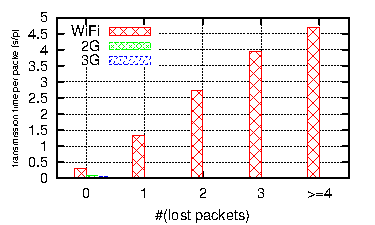
\includegraphics[width=0.8\linewidth]{web_loss_finish_time}
\caption{Transmission time per packet under different number of lost packets.}
\label{fig:web_loss_finish_time}
\end{figure}

Next, we investigate how much packet loss events could increase finish time. Figure~\ref{fig:web_loss_finish_time} shows the average finish time of web search flows under different number of lost packets. In the figure, flows are grouped by counting how many lost packets in each flow, and the average finish time in each group is calculated. When there is no packet loss, the average finish time of flows in WiFi network is about 1 second, while that of flows in 3G network is only 0.3 second, which is induced by smaller RTT in 3G network. When the number of lost packets is 1, the finish time in WiFi network increases to 2.6 second, while that of flows in cellular network hardly increases, compared with those without packet loss. When the number of lost packets increases to 3 or more, the finish time of flows in both networks increases greatly.

\subsection{Impact of timeout retransmission}

\begin{table}[th]
\caption{The average number of timeout retransmissions under different number of lost packets.}
\label{tab:web_rto_ratio}
\centering
\renewcommand{\arraystretch}{1.1}
\begin{tabular}{l|c|c|c}
	\toprule
	\#(lost pkts)  & 1 & 2 & $\ge$ 3 \\
	\midrule
	WiFi & 0.35 & 0.41 & 0.93 \\
	\hline
	3G & 0.02 & 0.02 & 0.06 \\
	\bottomrule
\end{tabular}
\end{table}

To understand how each packet loss impact finish time, we distinguish timeout retransmission from fast retransmit for each retransmission of lost packet. After that, we count the average number of timeout retransmissions in the flows within each group classified above, which is shown in Table~\ref{tab:web_rto_ratio}. From the table, when the number of lost packets is 1, there are much less timeout retransmissions in flows in 3G network, compared to those in WiFi network. This could explain why the finish time of flows in WiFi network increases a lot, while that of flows in 3G network does nearly not increase. Furthermore, the finish time under packet loss in each network is almost proportional to the average number of timeout retransmissions in that group. This indicates that when there is packet loss, timeout retransmission dominates the finish time in web search flows.

\begin{figure}[th]
\centering
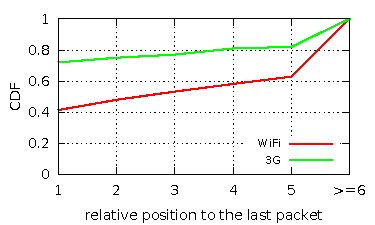
\includegraphics[width=0.8\linewidth]{web_rto_pos}
\caption{Position of timeout retransmission occurs in flows.}
\label{fig:web_rto_pos}
\end{figure}

Next, we investigate how timeout retransmission is triggered by inspecting where they occur. Figure~\ref{fig:web_rto_pos} shows the position of timeout retransmission occurs in flows. In the figure, the values in the x-axis represents the relative position to the last packet, where 1 means the last packet. The lines show the cumulative fraction of timeout retransmission occurs in the last $n$ packets, where $n$ is the value in the x-axis. From the figure, timeout retransmission in the last 3 packets occupies more than 53\% of all timeout retransmission. This coincides with the study in \cite{flach2013reducing} that packet loss at flow tail is likely to trigger timeout retransmission due to insufficient number of duplicate acknowledgments. As 47\% of flows in WiFi network experience timeout retransmission not at the tail of flow, which is much higher than those in 3G network.

Essentially, there are two scenarios that would trigger timeout retransmission. The first case is that sender does not receive sufficient number of duplicate acknowledgments (dupacks). The insufficient number of dupacks could be induced by various reasons. Besides packet loss at flow tail, packet loss under small congestion window, as well as packet delay may also trigger timeout retransmission. Packet delay is that the data packet is delayed, yet sender transmits the packet due to not receiving acknowledgment until RTO is triggered. The second case is that sender could only rely on timeout retransmission for recovery if a retransmitted packet is dropped (noted as \emph{double\_retransmission}). We propose a simple strategy to determine how each RTO is triggered in Algorithm~\ref{alg:rto}.

\begin{algorithm}
	\caption{Process of determining the cause of RTO.}
	\label{alg:rto}
	\begin{algorithmic}[1]
		\Procedure{ParseRTO}{$RTO$}
			\If {position to tail $\le$ 3}
				\State \textbf{return} $ tail\_retransmission$
			\ElsIf {spurious retransmission}
				\State \textbf{return} $ packet\_delay$
			\ElsIf {packet has been retransmitted}
				\State \textbf{return} $ double\_retransmission$
			\Else
				\State {// \#(dupacks) + \#(in-flight packets) $\le$ 3}
				\State \textbf{return} $ small\_cwnd$
			\EndIf
		\EndProcedure
	\end{algorithmic}
\end{algorithm}

\begin{table}[th]
\caption{The ratio of timeout retransmissions in each type.}
\label{tab:rto_type}
\centering
\renewcommand{\arraystretch}{1.1}
\begin{tabular}{l|c|c|c|c}
\toprule
& tail retx & double retx & pkt delay & small cwnd \\
\midrule
WiFi & 53.2\% & 17.8\% & 7.3\% & 21.5\% \\
\hline
3G & 77.1\% & 9.1\% & 3.0\% & 10.8\% \\
\bottomrule
\end{tabular}
\end{table}

According to the algorithm, we determine how many timeout retransmissions belongs to each type. Table~\ref{tab:rto_type} shows the ratio in each type. From the table, flows in WiFi network suffer more from double retransmission and retransmission in small congestion window, which are induced by higher packet loss rate. The diversity of reasons that trigger timeout retransmission may hinder the effort to reduce latency in short flows, like TLP~\cite{flach2013reducing}.

\subsection{Summary of web search analysis}

The key observations on web search flows are summarized below.

\begin{itemize}
	\item Compared to the impact of RTT on voice recognition flow, RTT has limited affect on the transmission time per packet in web search.
	\item More than 50\% of flows spend 30\% of their total time on establishing connections.
	\item Flows in WiFi network spend tens of times more than estimated time in congestion avoidance due to timeout retransmission.
	\item Most of timeout retransmissions in both networks are induced by packet loss at flow tail. However, about 18\% of timeout retransmissions in WiFi are induced by loss of retransmitted packet.
\end{itemize}
